\subsection{$\overline{K_n \cup claw \: m}$}
La familia consiste en un grafo $K_n$ y un grafo claw o estrella formado por un nodo y m nodos adyacentes, 
unidos de forma disjunta, que es luego complementado.
\begin{figure}[H]
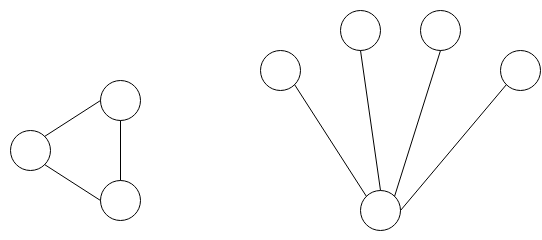
\includegraphics[width=80mm]{K3UC4.png}
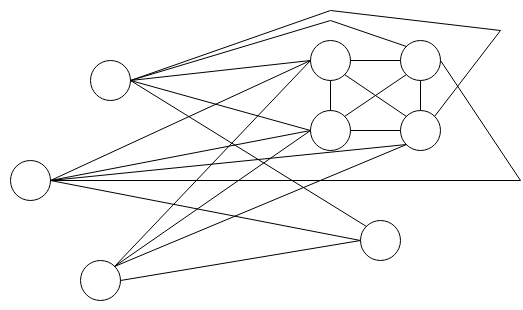
\includegraphics[width=80mm]{K3UC4Complemento.png}
\caption{Ejemplificación: La figura de la izquierda corresponde a $K_3$ $\cup$ $claw$ $4$, 
la figura derecha $\overline{K_3 \cup claw \: 4}$}
\label{overflow}
\end{figure}

\subsection{Grafo Completo K_n}
Un grafo completo es un grafo simple donde cada par de vértices está conectado por una arista.
Un grafo completo de n vértices tiene n(n-1)/2 aristas.
Es un grafo regular con todos sus vértices de grado n-1.

\begin{figure}[H]
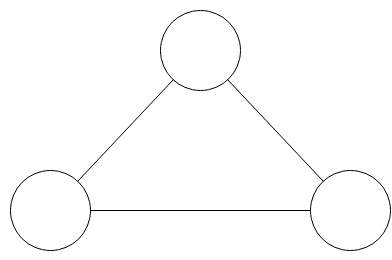
\includegraphics[width=80mm]{K3.png}
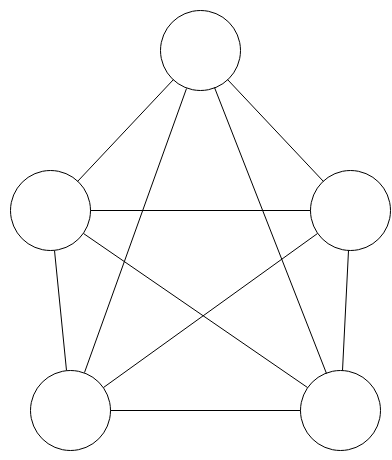
\includegraphics[width=80mm]{K5.png}
\caption{La figura de la izquierda corresponde a un grafo K_3 y la figura derecha a un grafo K_5}
\label{overflow}
\end{figure}

\subsection{Grafo Bipartito Completo K_n,_m}
Un grafo bipartito completo es aquel grafo bipartito en el que todos los vértices de la partición V_1 están conectados a todos los vértices de la partición V_2 y viceversa.

Donde un grafo bipartito es un grafo G=(V,E) cuyos vértices se pueden separar en dos conjuntos disjuntos V_1 y V_2, es decir, tal que se cumple:
V_1 $\cup$ V_2 = V
V_1 $\cap$ V_2 = $\emptyset$
de manera que las aristas sólo pueden conectar vértices de un conjunto con vértices del otro; es decir:
$\forall$ u_1,u_2 \in V_1, \forall v_1,v_2 \in V_2 no existe ninguna arista e=(u_1,u_2) ni e=(v_1,v_2).

\begin{figure}[H]
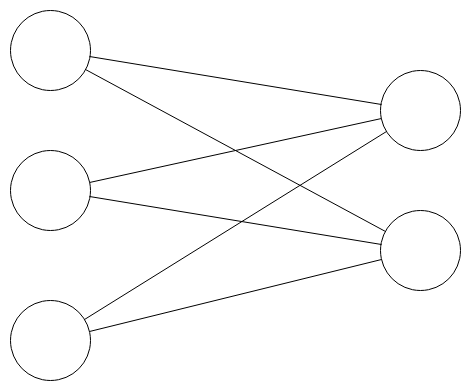
\includegraphics[width=80mm]{K3_2.png}
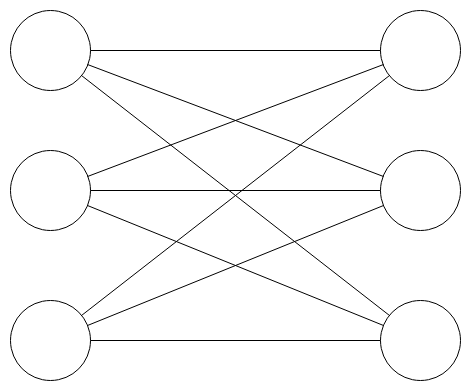
\includegraphics[width=80mm]{K3_3.png}
\caption{La figura de la izquierda corresponde a un grafo bipartito completo K_3_2 y la figura derecha a un grafo bipartito completo K_3_3}
\label{overflow}
\end{figure}


\subsection{Grafo Lattice L_m_n}
Un grafo Lattice es el producto cartesiano de dos grafos completos K_m y K_n.

\begin{figure}[H]
\includegraphics[width=80mm]{.png}
\includegraphics[width=80mm]{.png}
\caption{La figura de la izquierda corresponde a un grafo Lattice L y la figura derecha a un grafo Lattice L}
\label{overflow}
\end{figure}